\documentclass[draftclsnofoot,onecolumn]{IEEEtran}

\usepackage{amsmath,amsthm,amssymb}
\usepackage{graphicx}
\graphicspath{{/home/jingle/figures/}} %path to graphs
\usepackage{subfigure}

\usepackage{url}
\usepackage{cite}

% correct bad hyphenation here
\hyphenation{op-tical net-works semi-conduc-tor}

\begin{document}

\title{Traf: A Camera Based System for Traffic Flow Analysis}
\maketitle
\author{fsb}

\begin{abstract}

In this paper, we present a camera based system(Traf) to count automotive vehicles for traffic flow analysis use. The system employs the method of background subtraction by comparing differences between foreground and background. The background model is initialed by averaging first 50 frames, and adapted to environment change by introducing an adapting parameter $\lambda$. Compared to state-of-art method, it is more robust, adaptive and economical.

\end{abstract}


%--------------------------------------------------------------------------------
% what and why ?
\section{Introduction}

%================================================================================

% how?
\section{System Design}
	%============================================================================
	\subsection{Overview}
	The system consists of 3 main modules, video collector, vehicle counter and flow analyzer as Fig \ref{fig:sysDiagram}. Video collector is designed to collect the original video sources and transform them into a unified format for further use. Flow analyzer is designed to calculate the result and provide suggestion for traffic use. The vehicle counter is the core module of the system, which is further divided into 4 steps as, detector, tracker, follower and generator. 
	
	\begin{figure}[!h]
	\centering
	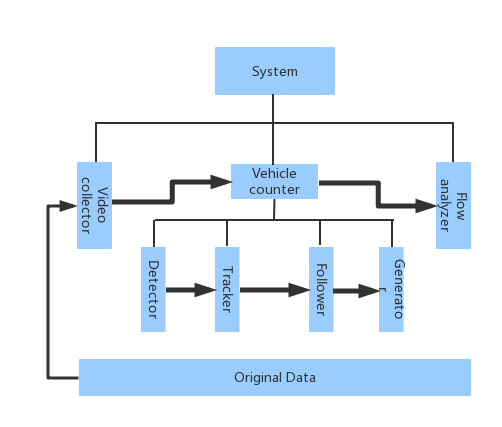
\includegraphics[width=0.8\linewidth]{diagram1.png} 
	\caption{System diagram:Video collector - Vehicle counter - Flow analyzer}
	\label{fig:sysDiagram}
	\end{figure}
	
	
	%============================================================================
	\subsection{Background Subtraction}
	As the monitoring camera is deployed with a fixed position, videos collected from this kind of devices would have a stable background. And the automobile vehicles forms the foreground motions. Hence, content of each frame image contains two parts, foreground and background. To detect the vehicles, we utilize background subtraction method, which can be described as:
	\begin{equation}
	F = I  - B
	\label{eq:backgroundSubtraction}
	\end{equation}
	Where $I$ is derived from frame image, $B$ is the corresponding background, and $F$ is hence the detected foreground.
	
	Frame images from video usually have more than one channel, and they may vary from different types and sizes. This makes it hard or impossible for directing subtraction calculation. Hence, we introduce a collector module to unify the original frame images, as Fig.\ref{fig:unifyDiagram}
	\begin{figure}[!h]
	\centering
	\subfigure[Original frame image]{
	\includegraphics[width=0.22\linewidth]{frameImg.jpg}}
	\subfigure[8 bits unsigned char with single channel]{
	\includegraphics[width=0.22\linewidth]{frameImgGry.jpg}}
	\subfigure[background model]{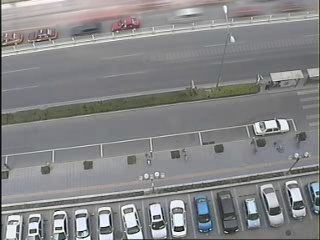
\includegraphics[width=0.22\linewidth]{InitBackgroudFile.jpg}}	
	\subfigure[Filter Guassian noise]{
	\includegraphics[width=0.22\linewidth]{guassian.jpg} }
	\caption{Unifying frame image:transform the original image to 8 bits unsigned char with single channel}
	\label{fig:unifyDiagram}
	\end{figure}
	
	After unifying operation, we do background subtraction, and get the foreground image $F$ as Eq.\ref{eq:backgroundSubtraction}. $F$ is mainly consisted of 2 area, the black and the gray. They stands for the background and the foreground separately. However, the gray parts is distributed all the image, making it hard for automobile vehicle detection. Ideally, the gray area of $F$ should gather together as an island. But due to camera performance, environment disturbance and so on, the image carries noise. Even worse,some parts of automobile vehicle may have coincident color with the background overlapping, this would results in gabs and separations.
	\begin{equation}
	  mask=sign(v)=\left\{
	   \begin{aligned}
	   	1, v \geq \delta \\
	   	0, v < \delta \\
	   \end{aligned}
	   \right.
	   \label{eq:foreMask}
	\end{equation}		
	To solve the problem above, we take following strategies as Fig.\ref{fig:preDetection}. First, we employs a Guassian filter with 4*4 size window to reduce noise. Second, we transform the result into binary image with Eq.\ref{eq:foreMask}, the result $Mask$ may consists of several neighbor areas. To make it a nice mask for describing automobile vehicles' shape and position, we employed dilation. Finally, we applied erosion for a better result. 
	\begin{figure}[!h]
	\centering
	\includegraphics[width=0.45\linewidth]{diagram2.png} 
	\caption{Diagram:Frame image pre-Detection diagram}
	\label{fig:preDetection}
	\end{figure}
	
	\begin{figure}[!h]
	\subfigure[Filter Guassian noise]{
	\includegraphics[width=0.22\linewidth]{guassian.jpg} }
	\subfigure[Binary image]{
	\includegraphics[width=0.22\linewidth]{binary.jpg} }
	\subfigure[Dilation]{
	\includegraphics[width=0.22\linewidth]{dilation.jpg} }
	\subfigure[Erosion]{
	\includegraphics[width=0.22\linewidth]{erosion.jpg} }
	\centering
	\caption{Guassian Filter - Binary Image - Dilation - Erosion}
	\label{fig:preDetection}
	\end{figure}




	\subsection{Background Model}
	Frame images consists of two parts, foreground and background. If there were no automobile vehicles within the frame image, the background is hence equal to the frame image. But this is not always the case, as the automobile vehicles are running on the road from time to time. Even worse, background may change due to light, wind and so on. So a steady background model is essential to the robustness of the system.
	Traf first builds the initial background model by averaging first 50 frame images. The result is shown as Fig \ref{fig:backgroundModel}.
%	\begin{figure}[!h]
%	\centering
%	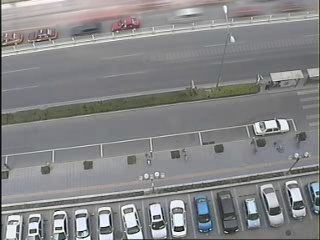
\includegraphics[width=0.4\linewidth]{InitBackgroudFile.jpg} 
%	\caption{Background model construction}
%	\label{fig:backgroundModel}
%	\end{figure}
	 	
	To adapt to environment change, Traf employs an adaptive parameter $\lambda$ as equation \ref{eq:adaption}.
	\begin{equation}
	M_{t} = (1-\lambda)M_{t-1} + \lambda B_{t}
	\label{eq:adaption}
	\end{equation}
	where $M_t$ and $M_{t-1}$ are the background model at time $t$ and $t-1$, $B_{t}$ is the background derived from frame image at time $t$.
	\begin{eqnarray}	
	F_{t}=&I_{t} - M_{t-1}	\\
	B_{t}=&y(F_{t})*M_{t-1}+(1-y(F_{t}))I_{t}
	\end{eqnarray}
Item $B_{t}$ is built from the mask of foreground and background model at time $t$. The mask is derived from a sign function as:
	\begin{equation}
	  y=sign(F)=\left\{
	   \begin{aligned}
	   	1, F \geq \epsilon \\
	   	0, F < \epsilon \\
	   \end{aligned}
	   \right.
	\end{equation}			
	
				
	
	\subsection{Motion}
	After preview operations, $Mask$ becomes a binary image consists of white islands and black background. The white symbolizes vehicle cars within foreground. The following process is to identify these islands, or motion detection. To count the vehicle correctly, we need also to track each detected vehicles.
	
	\subsubsection{Detection}
	We implement detection by detect the contour of the island, then we calculate the area of the island. Considering the size and the shape of a automobile vehicle, it's obviously that islands with small area should be expelled. After the vehicle has been detected, we draw a rectangular box to hold it for further identification and tracking.
	
	
	\subsubsection{Tracking}
	We employ Kalman-filter to tracking the detected car, this is done by building a moving model and estimating position for each frame.	%============================================================================


	%============================================================================
	\subsection{Traffic Flow Analysis}
	
	
	
% compare and check	
\section{Implementation and Evaluation}
	\subsection{Setup}
	\subsection{Methodology}
	\subsection{Result}



\section{Conclusion}


\end{document}